\documentclass{article}
\usepackage{amssymb}

\usepackage{neurips_2026}
\usepackage{amssymb}

\usepackage[T1]{fontenc}
\usepackage[utf8]{inputenc}
\usepackage{microtype}
\usepackage{graphicx}
\usepackage{booktabs}
\usepackage{array}
\usepackage{amsmath}
\usepackage{enumitem}
\usepackage{xcolor}
\usepackage{hyperref}
\usepackage{float}
\usepackage{subcaption}
\usepackage{multirow}
\usepackage{nicefrac}
\usepackage{wrapfig}

\newcommand{\pless}{P-less}
\newcommand{\best}[1]{\textbf{#1}}
\newcommand{\Qfour}{Q\textsubscript{4}}

\title{Long-Context Generation Is a Sampling Problem\\(When You Turn Up the Heat)}

\author{
  Anonymous Author(s)
}

\begin{document}
\maketitle


\begin{abstract}
Long generations from open-weight language models drift into repetition and incoherence, and the usual fix is more training. We show that the sampler, the rule that turns a model's next-token probabilities into an actual token, is a powerful and free lever on long-context generation, and we identify the one property that decides which samplers work. Across 23 open-weight models from 1B to 122B parameters, three published long-writing benchmarks, forced 16K-token generation, and coding agents on SWE-bench Verified, the result is the same: once the sampling temperature rises above 1, samplers whose candidate set stays small and stable degrade little or not at all, while samplers that let low-probability tokens in fall apart. Coding agents using top-$p$, top-$k$ or Top-H at $T{=}2$ resolve 0 of 100 GitHub issues; the same agents using top-$n\sigma$ resolve 46--62, winning every disputed issue on three Qwen3.5 models. On LongBench-Write, top-$n\sigma$ scores 80.6 at $T{=}2$ against 21 for top-$p$. Measuring the tokens each rule admits per step explains why: at one real decoding step, raising $T$ from 1 to 2 takes top-$p$ from 4 candidate tokens to 51,845, while top-$n\sigma$ keeps the same 3. A causal test confirms it: deciding the candidate set at $T{=}1$ and applying temperature only inside it rescues Top-H, min-$p$ and P-less. At the default $T{=}1$ the truncation rules reach similar quality and resolve rates, so the choice matters most when long and agentic generation turn up the heat, through exploration, best-of-$n$ selection, or escaping repetition.
\end{abstract}

%% ====================================================================
\section{Introduction}
%% ====================================================================

Open-weight language models now accept and nominally generate very long sequences~\citep{dubey2024llama3,yang2024qwen2}, yet the back half of a long sample often dissolves into repeated phrases and loops~\citep{holtzman2020curious,welleck2020neural,fu2021theoretical}. The usual remedies are retraining and long-output fine-tuning~\citep{bai2025longwriter}. This paper is about a cheaper lever that every deployment already has: the sampler.

\paragraph{Sampling in one paragraph.}
At every step a language model outputs a probability for each of the $\sim$100K tokens in its vocabulary. A \emph{sampler} turns those probabilities into one chosen token. \emph{Temperature} $T$ reshapes them first: $T{<}1$ sharpens the distribution toward the most likely token, and $T{>}1$ flattens it so that less likely tokens gain probability. A \emph{truncation rule} then throws away the unlikely tokens and samples from the survivors, the \emph{candidate set}. Rules differ in how they decide what is unlikely: top-$k$ keeps a fixed number of tokens~\citep{fan2018hierarchical}, top-$p$ keeps enough tokens to cover a fixed share of probability~\citep{holtzman2020curious}, and newer rules such as min-$p$~\citep{nguyen2024minp}, top-$n\sigma$~\citep{tang2024topnsigma}, Top-H~\citep{baghaei2025toph} and P-less~\citep{tan2025pless} adapt to the shape of each step's distribution.

\paragraph{The question.}
Long and agentic generation regularly push models to temperatures above 1: to diversify long texts, to explore in best-of-$n$ selection and reinforcement-learning rollouts, or simply to break out of a repetition loop. We ask which samplers survive that regime and why. Figure~\ref{fig:teaser} previews the answer. At a real decoding step, raising the temperature from 1 to 2 leaves top-$n\sigma$ with the same 3 candidate tokens and min-$p$ with 8, but lets top-$p$ admit 51,845. Coding agents behave accordingly: at $T{=}2$, every top-$p$ and Top-H Qwen3.5 agent fails every task, while top-$n\sigma$ agents solve 46--72\% of them.

\begin{figure}[t]
\centering
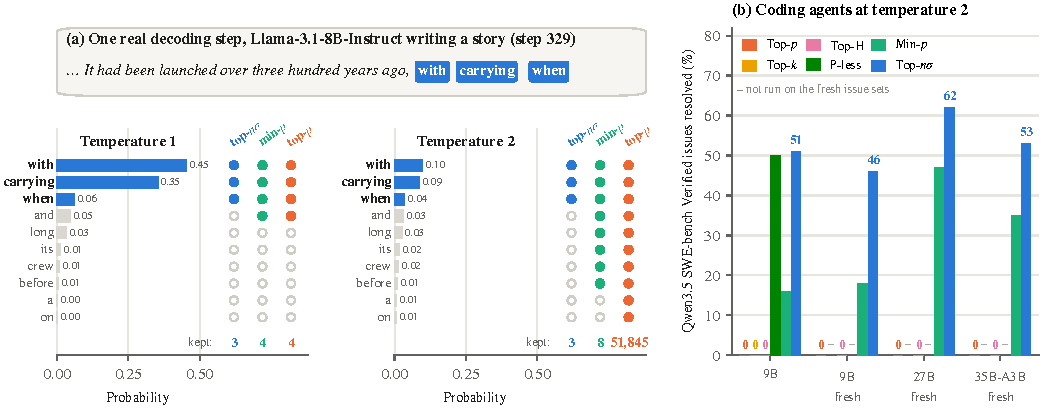
\includegraphics[width=\textwidth]{figures/fig_teaser.pdf}
\caption{\textbf{The rule that decides what counts as unlikely decides whether a model survives high temperature.} (a) A real next-token distribution from Llama-3.1-8B in the middle of a story (step chosen by a fixed rule, Appendix~\ref{app:numbers}). Blue bars are the tokens top-$n\sigma$ keeps. Raising $T$ from 1 to 2 flattens the distribution: top-$n\sigma$ still keeps the same 3 tokens and min-$p$ grows to 8, but top-$p$ 0.9 now needs 51,845 tokens to cover 90\% of the probability. (b) SWE-bench Verified issues resolved by coding agents at $T{=}2$ (100 issues per bar). Top-$p$ and Top-H agents resolve none; top-$n\sigma$ agents resolve 46--62\%.}
\label{fig:teaser}
\end{figure}

\paragraph{Findings.}
\begin{enumerate}[leftmargin=*,nosep]
\item \textbf{Small, stable candidate sets keep agents and long texts working when temperature rises.} Coding agents using top-$n\sigma$ win every disputed SWE-bench issue against top-$p$ at $T{=}2$, on three Qwen3.5 models, on the original issues and on 100 fresh ones (Section~\ref{sec:agentic}). The same ranking holds on Arena-Write, LongBench-Write and WritingBench (Section~\ref{sec:bench}) and position by position through forced 16K-token generations on ten models from 1B to 120B (Section~\ref{sec:r1}).
\item \textbf{The candidate set predicts which samplers survive:} a rule survives high temperature when the set it actually admits is small at $T{=}1$ and does not balloon as $T$ rises. We measure it at every decoding step (Section~\ref{sec:mechanism}) and map it across 22 settings, seven temperatures and eight models (Section~\ref{sec:map}).
\item \textbf{A causal test.} Fixing the candidate set at $T{=}1$ and applying temperature only inside it removes the temperature cliff for Top-H, min-$p$ and P-less (Section~\ref{sec:ablation}).
\item \textbf{The ``full-distribution-aware'' label does not describe one mechanism.} Top-H reads a global statistic, but its set still grows with temperature, so it holds up to about $T{=}1.5$ and collapses like top-$p$ by $T{=}2$; top-$n\sigma$ is provably temperature invariant (Section~\ref{sec:method}).
\end{enumerate}

%% ====================================================================
\section{Background and Related Work}
\label{sec:related}
%% ====================================================================

\paragraph{Truncation samplers.}
Beyond the rules above, locally typical sampling~\citep{meister2023locally}, $\eta$-sampling~\citep{hewitt2022truncation}, Mirostat~\citep{basu2021mirostat} and XTC~\citep{weidmann2024xtc} adapt the candidate set in other ways. Top-$n\sigma$, Top-H and P-less condition the candidate set on statistics of the whole distribution and have been grouped as ``full-distribution-aware''.

\paragraph{Text degeneration.}
Neural text generation is prone to repetition during extended generation~\citep{holtzman2020curious,welleck2020neural,fu2021theoretical}. Repetition penalties~\citep{keskar2019ctrl}, diversity objectives~\citep{li2016diversity}, the DRY penalty~\citep{weidmann2024dry} and contrastive search~\citep{su2022contrastive,su2023contrastive} target the same symptom. We study the base truncation rule and treat penalties in Appendix~\ref{app:extra}.

\paragraph{Sampler evaluation and long-context evaluation.}
A controlled thirteen-model study finds that truncation samplers change short-answer accuracy mainly when high temperature degrades a model~\citep{larosa2026fragility}. We find the same regime governs long-context and agentic generation, and we supply the mechanism. Long-context ability is usually measured through retrieval and comprehension~\citep{bai2024longbench,hsieh2024ruler,shaham2023zeroscrolls}, and long-output ability through benchmarks such as LongBench-Write~\citep{bai2025longwriter}. LLM judges~\citep{zheng2023judging,li2024generative} make it practical to score long outputs window by window.

%% ====================================================================
\section{How Each Sampler Responds to Temperature}
\label{sec:method}
%% ====================================================================

Let $\mathbf{z}\in\mathbb{R}^{|V|}$ be the logits at one step, $p=\mathrm{softmax}(\mathbf{z}/T)$ the tempered distribution, and $\mathcal{C}\subseteq V$ the candidate set. Following HuggingFace, vLLM and SGLang, every rule is applied to the tempered distribution. Table~\ref{tab:glance} summarizes the rules we compare and how large their candidate sets actually are.

\begin{table}[t]
\centering
\caption{\textbf{The samplers at a glance.} The last column is the measured median number of tokens each rule admits per decoding step at $T{=}1$ and $T{=}2$ (first 2K tokens of the ten-model generations of Section~\ref{sec:r1}; full numbers in Table~\ref{tab:pool}).}
\label{tab:glance}
\small
\begin{tabular}{lll}
\toprule
Sampler & Keeps the tokens that\ldots & Tokens kept, $T{=}1 \to T{=}2$ \\
\midrule
Pure sampling & (all tokens) & entire vocabulary \\
Top-$k$ 50 & are among the 50 most likely & 51 $\to$ 51 \\
Top-$p$ 0.9 & together cover 90\% of the probability & 2 $\to$ about 90{,}000 \\
Top-H 0.4 & keep the set's entropy under 40\% of the full entropy & 1 $\to$ 54 \\
Min-$p$ 0.1 & have at least 10\% of the top token's probability & 1 $\to$ 14 \\
P-less & have at least the collision probability $\sum_v p(v)^2$ & 1 $\to$ 21 \\
Top-$n\sigma$ 1 & have logits within one standard deviation of the maximum & 1 $\to$ 1 \\
\bottomrule
\end{tabular}
\end{table}

\paragraph{Top-$n\sigma$} keeps every token within $n$ standard deviations of the maximum logit:
\begin{equation}
\mathcal{C}_{\text{n-sigma}} = \{v \in V : z_v \ge \max_{u} z_u - n \cdot \sigma(\mathbf{z})\}.
\label{eq:nsigma}
\end{equation}
\paragraph{P-less} keeps tokens at least as probable as two independent draws are to collide, $\mathcal{C}_{\text{p-less}} = \{v : p(v) \ge \sum_u p(u)^2\}$. \textbf{Top-H} admits tokens in descending probability until the entropy of the renormalized set reaches a fraction $\alpha$ of $H(p)$, with $\alpha{=}0.4$.

\paragraph{Temperature response.}
Dividing $\mathbf{z}$ by $T$ scales $\max_u z_u$ and $\sigma(\mathbf{z})$ equally, so the top-$n\sigma$ set is identical at every temperature~\citep{tang2024topnsigma}: temperature only reshapes the probabilities inside it. Top-$k$ is fixed by construction but admits its $k$ tokens even when the model is nearly certain. Every other rule thresholds on the tempered distribution, so its set grows as $T$ flattens $p$: slowly for min-$p$ and P-less, whose thresholds are tied to the head of the distribution, and quickly for top-$p$ and Top-H, whose thresholds are tied to cumulative mass and entropy. Top-H therefore ends up with top-$p$ rather than top-$n\sigma$ as temperature rises, although both Top-H and top-$n\sigma$ read a global statistic. The low-probability \emph{tail} that fast-growing rules admit is what high temperature turns into noise.

%% ====================================================================
\section{Experimental Setup}
\label{sec:setup}
%% ====================================================================

\paragraph{Models and implementation.}
We use 23 instruction-tuned open-weight models from 1B to 122B parameters. The ten-model core set is Llama-3.2-1B, Qwen2.5-1.5B, Qwen2.5-3B, Mistral-7B-v0.3, Llama-3.1-8B, Mistral-Nemo-12B, Qwen2.5-14B, Qwen2.5-32B, Llama-3.3-70B~\citep{dubey2024llama3,yang2024qwen2,jiang2023mistral} and gpt-oss-120b~\citep{openai2025gptoss}, and further studies add Qwen3.5 (9B, 27B, 35B-A3B, 122B-A10B), Qwen3.6-27B, Qwen3.8-27B, Gemma-4 (E4B, 12B, 31B), OLMo-3 (7B, 3.1-32B), Nemotron-3 (Nano-4B, Nano-30B-A3B) and GLM-4.5-Air. All runs use the released weights (bf16, and native MXFP4 for gpt-oss-120b) on NVIDIA H200 GPUs. Every sampler runs as one vLLM logits processor that replaces native sampling, is checked against its authors' reference code, and logs the candidate-set size at every step.

\paragraph{Benchmarks and protocols.}
Agentic coding uses SWE-bench Verified~\citep{jimenez2024swebench} with the mini-swe-agent harness~\citep{minisweagent,yang2024sweagent} and the official test harness. Long chain-of-thought coding uses LiveCodeBench v6~\citep{jain2025livecodebench}. Long-form writing uses LongBench-Write~\citep{bai2025longwriter}, WritingBench~\citep{wu2025writingbench} and the 75 English Arena-Write prompts~\citep{wu2026longwriterzero} that require at least 2,000 words, all with natural stopping. A controlled stress test forces eight fiction and eight non-fiction prompts (Appendix~\ref{app:prompts}) to 16K tokens with end-of-sequence disabled. Every experiment was pre-registered before its outputs were read.

\paragraph{Outcomes.}
An LLM judge (gpt-oss-120b) scores 1.5K-token windows at fixed depths from 1 to 10. A generation has a \emph{terminal loop} if, from some 1K-token window onward, at least 80\% of the remaining windows repeat 32-grams at least half the time, and it is \emph{healthy} if it has no terminal loop and every judged window has coherence at least 6. Agentic outcomes are objective: an issue counts as resolved only if the agent's patch passes the repository's tests. We compare samplers on the same instances with exact sign tests.

%% ====================================================================
\section{Results}
\label{sec:results}
%% ====================================================================

\subsection{At high temperature, only tight samplers keep coding agents working}
\label{sec:agentic}

Agentic coding is long-context generation at its most practical. An agent issues tens to a few hundred commands and edits per episode into a context of tens of thousands of tokens, and one malformed command can end the episode. Figure~\ref{fig:swe} shows SWE-bench Verified resolve rates for six Qwen3.5 configurations, and Table~\ref{tab:swe} gives paired comparisons with top-$p$ for the long-horizon setting (500 agent steps, 262K-token window).

\begin{figure}[t]
\centering
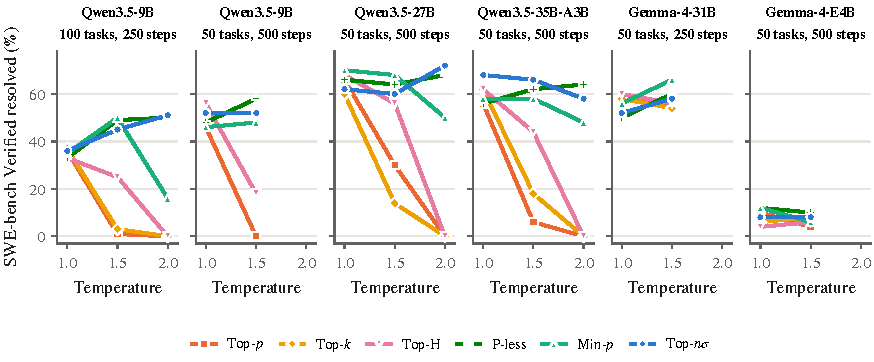
\includegraphics[width=\textwidth]{figures/fig_swe.pdf}
\caption{\textbf{Temperature-growing rules break coding agents; tight rules keep them working.} SWE-bench Verified resolve rate by temperature for Qwen3.5 agents, mini-swe-agent with the official test harness. The last two panels are 100 fresh issues disjoint from the first panel's. Other model families: Appendix~\ref{app:extra}.}
\label{fig:swe}
\end{figure}

\begin{table}[t]
\centering
\caption{\textbf{Long-horizon coding agents at $T{=}1.5$: min-$p$, P-less and top-$n\sigma$ win every disputed issue and keep their $T{=}1$ resolve rate.} Qwen3.5-9B, 500-step limit, 262K context, 50 issues. W/L: issues resolved by the sampler but not by top-$p$ 0.9 at the same $T$, and the reverse. $^{*}$: two-sided sign test $p<0.05$.}
\label{tab:swe}
\small
\begin{tabular}{lcccc}
\toprule
 & \multicolumn{2}{c}{$T{=}1.0$} & \multicolumn{2}{c}{$T{=}1.5$} \\
\cmidrule(lr){2-3} \cmidrule(lr){4-5}
Sampler & Resolved & W/L vs top-$p$ & Resolved & W/L vs top-$p$ \\
\midrule
Pure sampling & 46\% & 6/6 & 0\% & 0/0 \\
Top-$p$ 0.9 & 46\% & base & 0\% & base \\
Min-$p$ 0.1 & 46\% & 7/7 & 48\% & 24/0$^{*}$ \\
Top-H 0.4 & 56\% & 9/4 & 18\% & 9/0$^{*}$ \\
\pless{} & 48\% & 6/5 & 58\% & 29/0$^{*}$ \\
Top-$n\sigma$ 1 & 52\% & 9/6 & 52\% & 26/0$^{*}$ \\
\bottomrule
\end{tabular}

\end{table}

At $T{=}1$ every rule resolves about the same share of issues (33--37\% on the 100-issue grid, 46--56\% in the long-horizon setting). Raising the temperature separates them, and at $T{=}2$ completely. At $T{=}2$, top-$p$, top-$k$, Top-H and pure sampling resolve 0 of 100 issues on Qwen3.5-9B, because their commands degrade into malformed text within a few turns, while top-$n\sigma$ and P-less resolve 51 and 50 and win every disputed issue (51--0 and 50--0). The long-horizon agents also separate at $T{=}1.5$: min-$p$, P-less and top-$n\sigma$ resolve 48\%, 58\% and 52\% against 0\% for top-$p$, and win 24--0, 29--0 and 26--0 ($p<10^{-6}$).

The result replicates across models, issue sets and runs. On Qwen3.5-27B and Qwen3.5-35B-A3B, top-$p$, top-$k$, Top-H and pure sampling resolve nothing at $T{=}2$ while top-$n\sigma$ resolves 72\% and 58\% (36--0 and 29--0). On 100 fresh issues disjoint from the first set, top-$n\sigma$ resolves 46\%, 62\% and 53\% on the 9B, 27B and 35B-A3B models against 0\% for top-$p$ and Top-H, winning 46--0, 62--0 and 53--0. An independent repeat of the long-horizon grid gives top-$n\sigma$ 56\% and 60\% at $T{=}1.5$ and $2$ against 2\% and 0\% for top-$p$.

The same holds for long chain-of-thought coding without an agent. On LiveCodeBench v6 with Qwen3.8-27B in thinking mode (175 problems, two samples, 32K-token budget; Table~\ref{tab:lcb}), all rules score 61--64\% pass@1 at $T{\le}1$, and at $T{=}1.3$ top-$p$ 0.95 drops to 51\% while min-$p$, P-less, top-$n\sigma$ and Top-H hold 63\% and win 49--53 disputed problem-samples against 6--8 losses ($T{=}1.3$ is below Top-H's cliff). On Qwen3.6-27B, which exhausts its 32K budget on about half of all samples, top-$n\sigma$ again beats top-$p$ at $T{=}1.3$ (50.3\% against 46.3\%, 24--10, $p{=}0.02$; Table~\ref{tab:lcb36}).

\subsection{The same ranking on published long-writing benchmarks}
\label{sec:bench}

\begin{figure}[t]
\centering
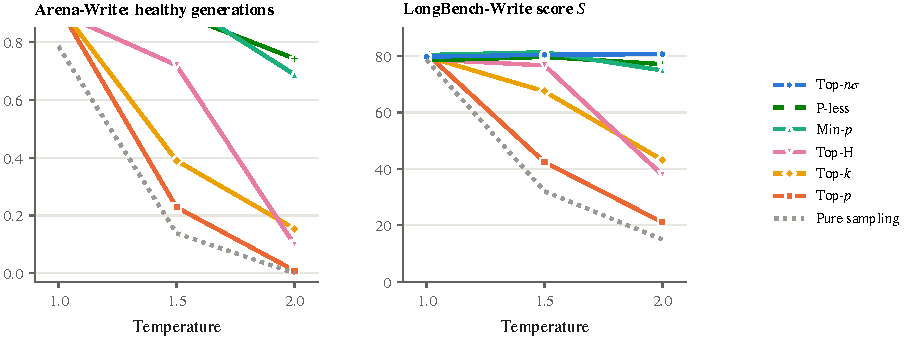
\includegraphics[width=\textwidth]{figures/fig_bench.pdf}
\caption{\textbf{On three published long-writing benchmarks, top-$n\sigma$ is the only rule unaffected by temperature.} Left: fraction of Arena-Write generations that are healthy, nine models including Llama-3.3-70B, gpt-oss-120b and Qwen3.5-122B-A10B. Middle: official LongBench-Write score. Right: WritingBench critic score (555 queries). Numbers in Table~\ref{tab:bench}.}
\label{fig:bench}
\end{figure}

Figure~\ref{fig:bench} reports Arena-Write~\citep{wu2026longwriterzero}, LongBench-Write~\citep{bai2025longwriter} and WritingBench~\citep{wu2025writingbench}, all with natural stopping. At $T{=}1$ the rules are close (90--93\% healthy on Arena-Write, LongBench-Write 78--81, WritingBench 6.8--6.9). At $T{=}2$ top-$n\sigma$ is unchanged on all three benchmarks (0.93 healthy, LongBench-Write 80.6, WritingBench 6.9), P-less and min-$p$ degrade moderately (0.74 and 0.69 healthy, LongBench-Write 77 and 75), and the tail-admitting rules collapse: Top-H, top-$k$ and top-$p$ are healthy on 0.10, 0.15 and 0.01 of Arena-Write generations and score 38, 43 and 21 on LongBench-Write, and top-$p$ scores 2.2 on WritingBench.

\subsection{Long generations, position by position}
\label{sec:r1}

\begin{figure}[t]
\centering
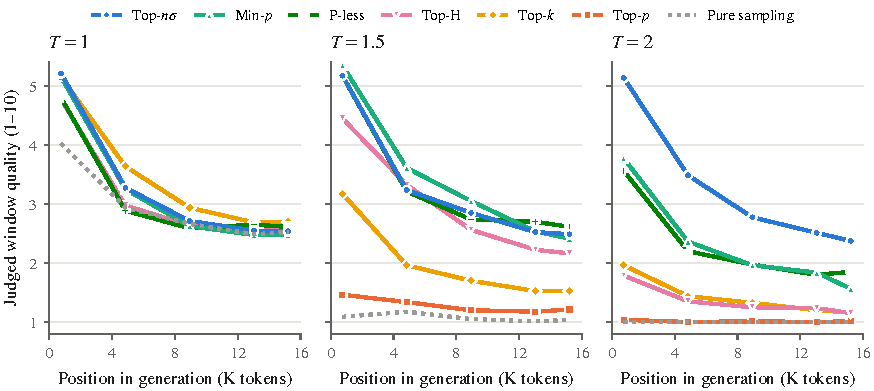
\includegraphics[width=\textwidth]{figures/fig_hero.pdf}
\caption{\textbf{At $T{=}2$, top-$n\sigma$ opens a long text as well as at $T{=}1$; tail-admitting rules produce word salad from the first window.} Judged quality of 1.5K-token windows by position in forced 16K-token fiction, ten models from 1B to 120B, 80 generations per line.}
\label{fig:hero}
\end{figure}

Forcing every model to write 16K tokens shows the effect along the length of a text (Figure~\ref{fig:hero}, Table~\ref{tab:r1}). At $T{=}1$ every truncation rule starts at 4.8--5.2 out of 10 and declines toward 2.5, so the sampler choice matters little for judged quality there. At $T{=}2$, top-$p$, top-$k$, Top-H and pure sampling open at 1.0--2.0 because the text is word salad from the first paragraph, min-$p$ and P-less open at 3.8 and 3.6, and top-$n\sigma$ opens at 5.1, the same as at $T{=}1$ (5.2). Top-$n\sigma$ is the only rule whose judged quality at $T{=}2$ matches its quality at $T{=}1$ (first window 5.1 against 5.2, last 2.4 against 2.5).

\subsection{Why: the candidate set each rule admits}
\label{sec:mechanism}

\begin{wrapfigure}{r}{0.44\textwidth}
\vspace{-12pt}
\centering
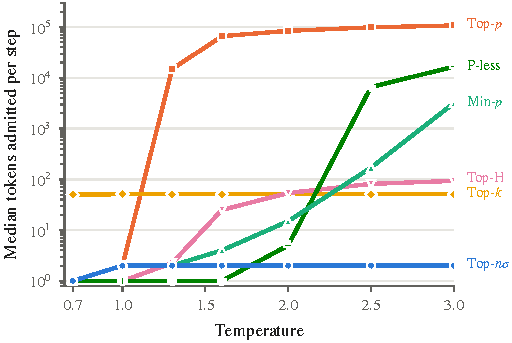
\includegraphics[width=0.44\textwidth]{figures/fig_pool.pdf}
\caption{\textbf{Top-$n\sigma$ is the only rule whose candidate set is both small and constant across temperatures.} Median tokens admitted per step (log scale), eight models, 64 generations per point.}
\label{fig:pool}
\vspace{-10pt}
\end{wrapfigure}
Our logits processor records how many tokens each rule admits at every step. Figure~\ref{fig:pool} and Table~\ref{tab:glance} show the answer. The top-$n\sigma$ set is provably invariant, and its measured median stays at 1 in the ten-model generations and 2 in the eight-model map at every temperature. By median, min-$p$ and P-less grow from 1 to 14 and 21 tokens between $T{=}1$ and $T{=}2$ and Top-H to 54, while top-$p$ grows to most of the vocabulary. Means are larger (min-$p$ and P-less occasionally admit thousands of tokens at $T{=}2$), and above $T{=}2.5$ their sets outgrow Top-H's. The faster a rule's candidate set grows, the more low-probability tokens temperature can promote, and those tokens are what turn a story into word salad and a shell command into a format error. Together with the size of the set at $T{=}1$ (top-$k$ never grows, but always admits about 50 tokens), this measurement separates the rules into the same groups that the benchmarks and agents do.

\subsection{Where each sampler stays usable}
\label{sec:map}

To check that this is a property of the rules and not of one hyperparameter, we map 22 settings across seven temperatures from 0.7 to 3.0 on eight models from five families, with 64 forced 8K-token generations per cell (Figure~\ref{fig:map}). Top-$n\sigma$ with $n\le1$, whose set is both invariant and small, holds a judged quality of 4.2--4.7 from $T{=}0.7$ all the way to $T{=}3.0$. Larger $n$ admits more of the tail at every temperature and brings a cliff back, and for the other families the hyperparameter moves the cliff. Top-$p$ falls below 1.5 by $T{=}1.6$ at every $p$. Min-$p$ survives higher temperatures as $p$ grows ($p{=}0.02$ collapses after $T{=}1.3$, $p{=}0.1$ after 1.6, and $p{=}0.3$ stays above 4 through $T{=}2.5$), at the cost of a tighter candidate set everywhere below.

\begin{figure}[t]
\centering
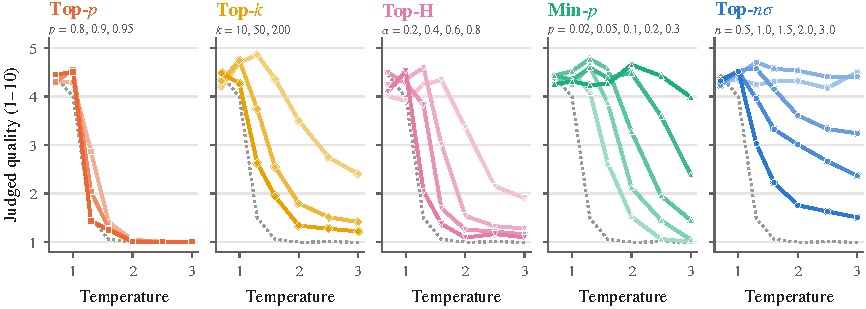
\includegraphics[width=\textwidth]{figures/fig_map.pdf}
\caption{\textbf{Top-$n\sigma$ with $n{\le}1$ keeps its judged quality all the way to $T{=}3$; every other setting has a cliff whose position the hyperparameter moves.} Mean judged window quality over eight models and 64 forced 8K-token generations per point. Lighter to darker lines follow the listed hyperparameter values. Dotted gray: pure sampling.}
\label{fig:map}
\end{figure}

\subsection{A causal test: fix the candidate set, remove the cliff}
\label{sec:ablation}

If high temperature hurts because it changes \emph{which} tokens are admitted, then deciding the candidate set at $T{=}1$ and applying temperature only inside it should remove the cliff. We pre-registered this test (Figure~\ref{fig:tl}, Table~\ref{tab:tl}). With the set fixed at $T{=}1$, Top-H, min-$p$ and P-less keep their $T{=}1$ quality through $t{=}3$ (4.1--4.6), where the standard order has collapsed them to 1.1--1.2. The rescue is specific to rules whose $T{=}1$ set already excludes the tail: in the ten-model generations top-$p$ at $T{=}1$ admits a mean of 73 tokens because it reaches deep into the tail at uncertain steps, and top-$k$ always admits about 50, so fixing their sets helps them only partly or not at all. Excluding the tail is the property that matters, and top-$n\sigma$ has it at every temperature by construction.

\begin{figure}[t]
\centering
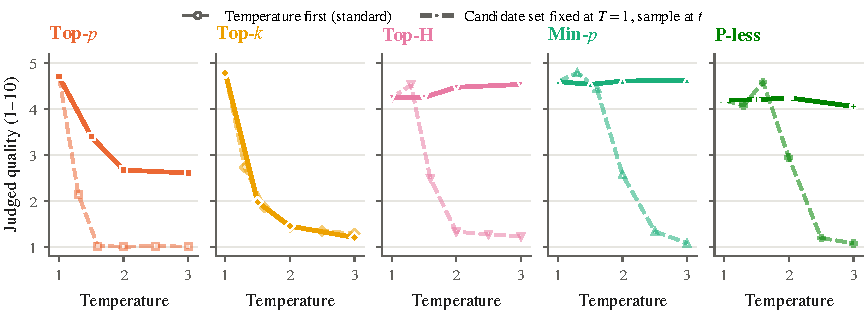
\includegraphics[width=\textwidth]{figures/fig_tl.pdf}
\caption{\textbf{Fixing the candidate set at $T{=}1$ removes the temperature cliff for Top-H, min-$p$ and P-less.} Dashed: standard order (temperature first). Solid: set decided at $T{=}1$, sampling at $t$. Four models, 32 generations per point.}
\label{fig:tl}
\end{figure}

\subsection{Robustness}
\label{sec:robust}

The forced-length and benchmark results replicate under every check in Appendix~\ref{app:robust}: a second seed on all ten core models; six newer models including GLM-4.5-Air and Qwen3.5-122B-A10B, where top-$n\sigma$ opens at 7.4 at $T{=}2$ against 1.7 for top-$p$; natural-length generation in which the model may stop and is asked to continue; and non-fiction. Among coding agents, Gemma-4-31B does not separate at $T{=}1.5$, as the mechanism predicts, because its top-$p$ set still holds about one token there (Appendix~\ref{app:extra}). A second judge from a different model family (GLM-4.5-Air) agrees with the first at Spearman $\rho{=}0.92$ on the 22 sampler-by-temperature cell means ($\rho{=}0.74$ on 8,796 individual windows).

%% ====================================================================
\section{Practical Guidance}
\label{sec:discussion}
%% ====================================================================

\paragraph{If you raise the temperature, use a rule that excludes the tail.}
A rule whose candidate set grows with $T$ couples two things a practitioner wants to control separately: how much randomness to inject among plausible tokens, and how far into the implausible tail to reach. Top-$n\sigma$ with $n\le1$ decouples them by construction. Min-$p$ with a larger $p$, or any tight rule whose set is decided at $T{=}1$, decouples them in practice.

\paragraph{Long and agentic generation is where this matters.}
At the default temperature the truncation rules we tested reach similar quality and resolve rates, so benchmarks run only at $T{=}1$ will not reveal these differences. Long generation keeps pushing models into the high-temperature regime, to diversify long texts, to explore in best-of-$n$ selection and reinforcement-learning rollouts, and to escape repetition. In that regime the sampler decides whether a long text stays readable or turns into word salad, and whether an agent keeps working at all.

\paragraph{Report what the sampler actually admits.}
Nominal hyperparameters hide the property that matters. Reporting the realized candidate-set size per step, as our processor does, would let sampler comparisons predict behavior across temperatures.

%% ====================================================================
\section{Conclusion}
\label{sec:conclusion}
%% ====================================================================

The sampler is a free and powerful control on long-context generation. Across 23 models, three long-writing benchmarks, forced 16K-token generation and coding agents, samplers whose candidate set stays small and stable degrade little or not at all when the temperature rises, and samplers that admit the low-probability tail fall apart: top-$n\sigma$ agents resolve 46--62\% of SWE-bench Verified issues at $T{=}2$ where top-$p$ agents resolve none. The realized candidate set, small at $T{=}1$ and stable as $T$ rises, predicts which rule is which, and fixing it at $T{=}1$ rescues the rules it can. Long-context generation is a sampling problem the moment you turn up the heat.

%% ====================================================================
\bibliography{refs}
\bibliographystyle{plainnat}


%% ====================================================================
\newpage
\appendix

\section{Additional analyses}
\label{app:extra}

\subsection{Behavior at the default temperature and under forced length}
At $T{=}1$ under forced 16K-token generation, top-$p$, min-$p$, Top-H, \pless{} and top-$n\sigma$ end in a terminal loop in 95--100\% of generations, the same rate as greedy decoding, and top-$k$ and pure sampling in 56\% and 41\% (Table~\ref{tab:r1}). Under our pre-registered definition, which requires no terminal loop and judged coherence of at least 6 in every window, at most 2.5\% of generations in any $T{=}1$ cell are healthy. What no setting buys is a healthy long generation. Under the pre-registered definition, no cell of the entire map is healthy in more than 31\% of generations, and top-$n\sigma$ $n{=}1$ still ends in a terminal loop in 44--69\% of generations at every temperature. Top-$n\sigma$ widens the range of usable temperatures. It does not fix collapse at length. Raising the temperature removes loops for the tail-admitting rules only by producing word salad, and top-$n\sigma$ still loops in 71\% of generations at $T{=}2$. The sampler therefore controls how a forced long generation behaves under temperature, not whether a model that tends to loop will loop.

\subsection{Repetition penalties and an escape floor}
\label{sec:stack}

If loops are the problem and tail-admission is the cost of escaping them, two additions to the sampler are natural: a repetition penalty, and a floor that always keeps the top two tokens so that a tight rule can never be greedy. We tested both on top of each tight and tail-admitting rule, on eight of the ten models, including Llama-3.3-70B and gpt-oss-120b (Table~\ref{tab:stack}). We had predicted that DRY~\citep{weidmann2024dry} combined with a tight rule at $T{\ge}1.5$ would raise judged quality by at least one point. That prediction failed. DRY cuts the loop rate at $T{=}1$ from 95--100\% to 27--38\% for every rule, but judged quality moves by at most 0.2 points in either direction at any temperature, because the penalty replaces verbatim loops with text that is varied but no better. The top-2 floor does almost nothing at $T{=}1$, and the reason is instructive: a second candidate with probability $10^{-6}$ is never sampled. Its effect appears only with temperature. At $T{=}2$, top-$n\sigma$ plus the floor nearly eliminates terminal loops (from 75\% to 2\%) while keeping its judged quality (3.3), and it is the only loop-free configuration at $T{=}2$ that is not word salad (top-$p$, Top-H, min-$p$ and \pless{} with the floor score 1.0, 1.3, 2.4 and 2.5). A tail-excluding rule, an escape floor and an elevated temperature together remove loops without admitting the noise tail. They do not yet produce good long text, because the quality ceiling of these models at 16K is low under every sampler. On Arena-Write with natural stopping (six models), where loops are already rare, the floor changes little: top-$n\sigma$ is healthy on 0.94 of generations at $T{=}2$ with the floor against 0.93 without, and the floor lowers \pless{} at $T{=}2$ (0.60 against 0.70).

In agentic coding the floor is harmful. Adding the top-2 floor of Section~\ref{sec:stack} to top-$n\sigma$ hurts agents (42\% and 22\%), even though it removes loops in fiction, because the floor admits a second token at every step, including steps where the agent must emit an exact command: format errors per episode rise from 0.04 to 1.4 at $T{=}1.5$ and from 0.06 to 9.6 at $T{=}2$. 

\subsection{Context depth}
\label{sec:depth}

The title invites a direct test: does a longer \emph{input} context push models into the regime where the sampler matters? We continued PG-19 novels~\citep{rae2019compressive} from depths of 2K, 16K and 64K tokens on six long-context models (and 128K on the three that support it) and measured both the model's entropy at $T{=}1$ and the judged quality gap between tail-excluding rules (min-$p$, \pless{}, top-$n\sigma$) and tail-admitting rules (top-$p$, top-$k$, Top-H, pure sampling) (Table~\ref{tab:depth}). The pre-registered answer is no. The gap is within 0.4 points of zero at $T{\le}1$ at every depth and 1.2--1.6 points at $T{=}1.3$ and $1.6$ at every depth, with no trend. Entropy at $T{=}1$ rises with depth on Qwen3.5-27B and Qwen3.5-35B-A3B (for example from 1.16 to 1.70 nats on the latter), is mixed on Qwen3.5-9B and Nemotron, near zero on Gemma-4-12B, and falls on Llama-3.1-8B. What makes long generation a sampling problem is not the length of the context the model reads. It is the length of what the model writes, which is where loops form and where temperature is needed to escape them.

\subsection{Other model families in agentic coding}
Gemma-4 is the exception that fits the mechanism. On Gemma-4-31B no rule separates at $T{=}1.5$, on the first 50 instances or on the 100 fresh ones (49--55\% for every rule, all $p{>}0.3$), and the candidate sets explain why: in Gemma-4-31B's forced-length generations (Table~\ref{tab:r10}), top-$p$ still admits a median of one token per step at $T{=}1.5$ (33 at $T{=}2$), where Qwen3.5-27B, OLMo-3.1-32B and Llama-3.1-8B admit 28,000--143,000. We attribute this to Gemma's soft-capped final logits, which keep the distribution peaked under temperature, though we did not isolate the cap experimentally. Gemma-4-E4B resolves at most 12\% under any rule, too few to compare. OLMo-3.1-32B could not be evaluated: under every rule, including at $T{=}1$, it emits several actions per turn and mini-swe-agent ends 95\% of its episodes (over 10 configurations) for repeated format errors, so it resolves no instances.

\begin{figure}[h]
\centering
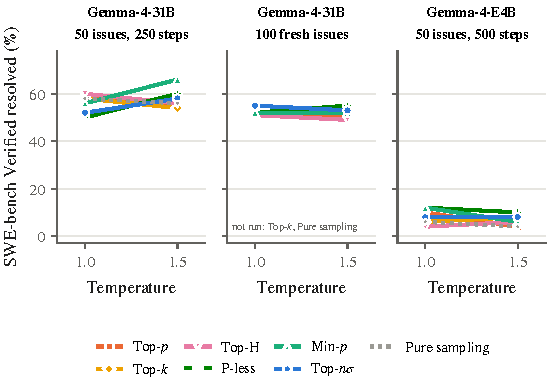
\includegraphics[width=0.6\textwidth]{figures/fig_swe_gemma.pdf}
\caption{SWE-bench Verified resolve rate for Gemma-4 agents.}
\label{fig:swe_gemma}
\end{figure}


\section{SWE-bench Verified: 100-instance grid}
\label{app:swe}

Qwen3.5-9B, mini-swe-agent, 250-step limit, 100 fixed instances, three temperatures. Following the SWE-bench convention, resolve rates are over all instances, and patches that are empty or that the official harness could not evaluate count as unresolved. W/L pairs each rule with top-$p$ 0.9 on the same instances. At $T{=}1$ every rule resolves 33--37\% and no paired comparison is significant ($p{>}0.6$). At $T{=}1.5$ and $2$ the tail-excluding rules win every disagreement.

\begin{table}[h]
\centering
\small
\begin{tabular}{lcccccc}
\toprule
 & \multicolumn{2}{c}{$T{=}1.0$} & \multicolumn{2}{c}{$T{=}1.5$} & \multicolumn{2}{c}{$T{=}2.0$} \\
\cmidrule(lr){2-3} \cmidrule(lr){4-5} \cmidrule(lr){6-7}
Sampler & Resolved & W/L vs top-$p$ & Resolved & W/L vs top-$p$ & Resolved & W/L vs top-$p$ \\
\midrule
Pure sampling & -- & -- & 0\% & 0/1 & 0\% & 0/0 \\
Top-$k$ 50 & -- & -- & -- & -- & 0\% & 0/0 \\
Top-$p$ 0.9 & -- & -- & 1\% & base & 0\% & base \\
Min-$p$ 0.1 & -- & -- & -- & -- & 16\% & 16/0$^{*}$ \\
Top-H 0.4 & -- & -- & -- & -- & 0\% & 0/0 \\
\pless{} & -- & -- & -- & -- & 50\% & 50/0$^{*}$ \\
Top-$n\sigma$ 1 & -- & -- & 45\% & 44/0$^{*}$ & 51\% & 51/0$^{*}$ \\
\bottomrule
\end{tabular}

\end{table}

\section{Forced-length replication in numbers}
\label{app:r1}

\begin{table}[h]
\centering
\caption{\textbf{Forced to 16K tokens, every sampler collapses at $T{=}1$. Raising $T$ changes how each one fails.} Ten models, eight fiction prompts, seed 1, 80 generations per cell. Loop: fraction of generations ending in a terminal loop. First / Last: judge overall score (1--10) for the first and final 1.5K-token windows.}
\label{tab:r1}
\small
\begin{tabular}{lccccccccc}
\toprule
 & \multicolumn{3}{c}{$T{=}1.0$} & \multicolumn{3}{c}{$T{=}1.5$} & \multicolumn{3}{c}{$T{=}2.0$} \\
\cmidrule(lr){2-4} \cmidrule(lr){5-7} \cmidrule(lr){8-10}
Sampler & Loop & First & Last & Loop & First & Last & Loop & First & Last \\
\midrule
Pure sampling & 0.41 & 4.0 & 2.5 & 0.03 & 1.1 & 1.0 & 0.00 & 1.0 & 1.0 \\
Top-$k$ 50 & 0.56 & 5.2 & 2.7 & 0.00 & 3.2 & 1.5 & 0.00 & 2.0 & 1.2 \\
Top-$p$ 0.9 & 0.95 & 5.2 & 2.5 & 0.05 & 1.5 & 1.2 & 0.00 & 1.0 & 1.0 \\
Min-$p$ 0.1 & 0.97 & 5.2 & 2.5 & 0.64 & 5.3 & 2.4 & 0.09 & 3.8 & 1.6 \\
Top-H 0.4 & 0.97 & 4.8 & 2.6 & 0.20 & 4.5 & 2.2 & 0.00 & 1.8 & 1.1 \\
\pless{} & 0.99 & 4.8 & 2.6 & 0.99 & 5.2 & 2.6 & 0.44 & 3.6 & 1.9 \\
Top-$n\sigma$ 1 & 1.00 & 5.2 & 2.5 & 0.90 & 5.2 & 2.5 & 0.71 & 5.1 & 2.4 \\
\midrule
Greedy & \multicolumn{3}{c}{1.00 / 4.8 / 2.5} &  &  &  &  &  &  \\
\bottomrule
\end{tabular}

\end{table}

\begin{table}[h]
\centering
\caption{LiveCodeBench v6, Qwen3.8-27B in thinking mode, 175 problems $\times$ 2 samples, 32K tokens, official tests in a sandbox. W/L: problem-samples solved by the rule but not by top-$p$ 0.95 at the same $T$, and the reverse. $^{*}$: sign test $p<0.05$.}
\label{tab:lcb}
\small
\begin{tabular}{lcccccc}
\toprule
 & \multicolumn{2}{c}{$T{=}0.6$} & \multicolumn{2}{c}{$T{=}1$} & \multicolumn{2}{c}{$T{=}1.3$} \\
\cmidrule(lr){2-3} \cmidrule(lr){4-5} \cmidrule(lr){6-7}
Sampler & pass@1 & W/L & pass@1 & W/L & pass@1 & W/L \\
\midrule
Top-$p$ 0.95 & 62.0 & base & 60.9 & base & 50.6 & base \\
Top-$n\sigma$ 1 & 63.4 & 14/9 & 63.7 & 22/12 & 63.4 & 53/8$^{*}$ \\
Min-$p$ 0.1 & 62.6 & 14/12 & 62.9 & 21/14 & 63.1 & 50/6$^{*}$ \\
\pless{} & 62.0 & 14/14 & 62.6 & 22/16 & 62.6 & 49/7$^{*}$ \\
Top-H 0.4 & 61.7 & 15/16 & 62.6 & 22/16 & 62.9 & 50/7$^{*}$ \\
\bottomrule
\end{tabular}

\end{table}

\begin{table}[h]
\centering
\caption{LiveCodeBench v6, Qwen3.6-27B in thinking mode, same protocol as Table~\ref{tab:lcb}. This model exhausts the 32K-token budget on 44--53\% of samples in every cell. At $T{=}0.6$, \pless{} and Top-H lose to top-$p$.}
\label{tab:lcb36}
\small
\begin{tabular}{lcccccc}
\toprule
 & \multicolumn{2}{c}{$T{=}0.6$} & \multicolumn{2}{c}{$T{=}1$} & \multicolumn{2}{c}{$T{=}1.3$} \\
\cmidrule(lr){2-3} \cmidrule(lr){4-5} \cmidrule(lr){6-7}
Sampler & pass@1 & W/L & pass@1 & W/L & pass@1 & W/L \\
\midrule
Top-$p$ 0.95 & 52.0 & base & 49.1 & base & 46.3 & base \\
Top-$n\sigma$ 1 & 52.9 & 20/17 & 51.4 & 18/10 & 50.3 & 24/10$^{*}$ \\
Min-$p$ 0.1 & 49.4 & 16/25 & 51.1 & 15/8 & 48.6 & 21/13 \\
\pless{} & 46.3 & 14/34$^{*}$ & 45.4 & 12/25$^{*}$ & 49.7 & 24/12 \\
Top-H 0.4 & 46.9 & 16/34$^{*}$ & 48.6 & 22/24 & 49.7 & 26/14 \\
\bottomrule
\end{tabular}

\end{table}

\section{Candidate sets and the temperature-last ablation in numbers}
\label{app:numbers}

\paragraph{Figure~\ref{fig:teaser}(a).} Llama-3.1-8B-Instruct decodes the science-fiction prompt greedily for 512 tokens. Among the steps whose top probability lies in $[0.3,0.7]$, we show the one with the median entropy (step 329, context ``\ldots It had been launched over three hundred years ago,'', $p_{\max}{=}0.45$, $H{=}1.43$ nats). Candidate-set sizes are computed exactly on the full 128K-token vocabulary.

\begin{table}[h]
\centering
\caption{\textbf{How the realized candidate set responds to temperature predicts how each sampler fails.} Median candidate-set size per decoding step over the first 2,048 tokens of the Table~\ref{tab:r1} generations (ten models). Singleton: fraction of steps at $T{=}1$ where only one token is admitted.}
\label{tab:pool}
\small
\begin{tabular}{lcccc}
\toprule
Sampler & $T{=}1.0$ & $T{=}1.5$ & $T{=}2.0$ & Singleton at $T{=}1$ \\
\midrule
Pure sampling & all & all & all & 0.00 \\
Top-$k$ 50 & 51 & 51 & 51 & 0.00 \\
Top-$p$ 0.9 & 2 & 41,508 & 89,581 & 0.46 \\
Min-$p$ 0.1 & 1 & 3 & 14 & 0.59 \\
Top-H 0.4 & 1 & 10 & 54 & 0.62 \\
\pless{} & 1 & 1 & 21 & 0.93 \\
Top-$n\sigma$ 1 & 1 & 1 & 1 & 0.52 \\
\bottomrule
\end{tabular}

\end{table}

\begin{table}[h]
\centering
\caption{\textbf{Deciding the candidate set at $T{=}1$ rescues Top-H, min-$p$ and \pless{} at high temperature, but not top-$p$ or top-$k$.} Mean judged window quality (1--10), four models, 32 forced 8K-token generations per cell. Temperature first: the standard order (Figure~\ref{fig:map}). Candidate set fixed at $T{=}1$: truncation on the untempered distribution, then sampling at temperature $t$ inside the kept set.}
\label{tab:tl}
\small
\begin{tabular}{lccccccc}
\toprule
 & $T{=}1$ & \multicolumn{3}{c}{Temperature first} & \multicolumn{3}{c}{Candidate set fixed at $T{=}1$} \\
\cmidrule(lr){3-5} \cmidrule(lr){6-8}
Sampler & & $T{=}1.6$ & $T{=}2$ & $T{=}3$ & $t{=}1.5$ & $t{=}2$ & $t{=}3$ \\
\midrule
Top-$p$ 0.9 & 4.7 & 1.0 & 1.0 & 1.0 & 3.4 & 2.7 & 2.6 \\
Top-$k$ 50 & 4.8 & 1.9 & 1.4 & 1.3 & 2.0 & 1.4 & 1.2 \\
Top-H 0.4 & 4.2 & 2.5 & 1.3 & 1.2 & 4.2 & 4.5 & 4.5 \\
Min-$p$ 0.1 & 4.6 & 4.4 & 2.6 & 1.1 & 4.5 & 4.6 & 4.6 \\
\pless{} & 4.2 & 4.6 & 2.9 & 1.1 & 4.2 & 4.2 & 4.1 \\
\bottomrule
\end{tabular}

\end{table}

\begin{table}[h]
\centering
\caption{Published long-writing benchmarks: Arena-Write and LongBench-Write (numbers behind Figure~\ref{fig:bench}) and WritingBench critic scores (1--10, six models).}
\label{tab:bench}
\small
\resizebox{\textwidth}{!}{\begin{tabular}{lcccccccccccc}
\toprule
 & \multicolumn{3}{c}{Arena-Write healthy} & \multicolumn{3}{c}{Arena-Write last window} & \multicolumn{3}{c}{LongBench-Write $S$} & \multicolumn{3}{c}{WritingBench} \\
\cmidrule(lr){2-4} \cmidrule(lr){5-7} \cmidrule(lr){8-10} \cmidrule(lr){11-13}
Sampler & $T{=}1$ & $T{=}1.5$ & $T{=}2$ & $T{=}1$ & $T{=}1.5$ & $T{=}2$ & $T{=}1$ & $T{=}1.5$ & $T{=}2$ & $T{=}1$ & $T{=}1.5$ & $T{=}2$ \\
\midrule
Pure sampling & 0.64 & 0.21 & 0.00 & 6.4 & 2.9 & 1.0 & 78.6 & 32.1 & 15.0 & 6.93 & 3.26 & 1.30 \\
Top-$k$ 50 & 0.74 & 0.41 & 0.23 & 6.8 & 4.8 & 3.1 & 79.8 & 67.4 & 43.1 & 7.07 & 6.13 & 4.54 \\
Top-$p$ 0.9 & 0.74 & 0.33 & 0.01 & 6.7 & 3.9 & 1.3 & 80.8 & 42.4 & 21.1 & 7.02 & 3.68 & 2.51 \\
Min-$p$ 0.1 & 0.74 & 0.76 & 0.52 & 6.7 & 6.8 & 5.5 & 80.3 & 81.3 & 74.9 & 7.00 & 7.09 & 6.42 \\
Top-H 0.4 & 0.73 & 0.70 & 0.15 & 6.5 & 6.5 & 2.8 & 78.8 & 76.6 & 37.8 & 6.93 & 6.92 & 3.76 \\
\pless{} & 0.72 & 0.73 & 0.67 & 6.6 & 6.6 & 6.3 & 78.4 & 79.6 & 77.1 & 6.94 & 6.96 & 6.82 \\
Top-$n\sigma$ 1 & 0.75 & 0.76 & 0.75 & 6.7 & 6.7 & 6.7 & 79.7 & 80.4 & 80.6 & 6.99 & 7.02 & 7.04 \\
\bottomrule
\end{tabular}
}
\end{table}

\section{Robustness, sampling stacks and context depth in numbers}
\label{app:robust}

\subsection{Natural-length continuation and non-fiction}
\label{sec:natural}

Forcing a model past the point where it wants to stop is an artificial stress, so we repeat the replication under a protocol closer to how long outputs are produced in practice. The model may emit end-of-sequence at any time, and each time it stops we append a ``Continue.'' turn, up to a 16K-token budget with 4K-token turns (Table~\ref{tab:r4}, nine of the ten models, excluding gpt-oss-120b).



Natural length helps every rule. At $T{=}1$ the final judged window rises from about 2.5 under forced length to 3.8--4.5, and the loop rate of top-$p$ falls from 0.95 to 0.50 and of top-$n\sigma$ from 1.00 to 0.39. The rules remain close on quality at $T{=}1$ (final-window means 3.8--4.5). \pless{} is the most loop-prone rule at $T{\le}1.5$ (0.89 and 0.76), consistent with its near-greedy candidate set. Raising the temperature reproduces the forced-length split. At $T{=}2$, top-$p$, top-$k$, Top-H and pure sampling score 1.0--2.1 on their first window, min-$p$ and \pless{} fall to 4.0--4.1, and top-$n\sigma$ holds 5.7, while still looping in 26\% of generations.

Non-fiction behaves the same way (Appendix~\ref{app:nonfic}, six models). At $T{=}1$ every rule ends at 3.3--3.6 on the final window, and at $T{=}1.5$ top-$p$ and top-$k$ fall to a first-window score of 3.1 and 4.4 while top-$n\sigma$ and min-$p$ hold theirs (6.3 to 6.6 and 6.3 to 6.5).

\subsection{Second seed, newer models, second judge}
\label{app:robust2}

Three checks support the forced-length results. A second seed on all ten models (80 generations per cell, Table~\ref{tab:r9}, Appendix~\ref{app:robust}) reproduces Table~\ref{tab:r1}: at $T{=}1$ top-$p$, min-$p$, Top-H, \pless{} and top-$n\sigma$ loop in 96--100\% of generations, and at $T{=}2$ top-$n\sigma$ opens at 5.3 while top-$p$ opens at 1.0. Six newer models (Gemma-4-31B, OLMo-3.1-32B, Qwen3.5-27B, Nemotron-3-Nano-30B-A3B, and the mixture-of-experts GLM-4.5-Air and Qwen3.5-122B-A10B, Table~\ref{tab:r10}) loop less often at $T{=}1$ (56--81\% for the five truncation rules) but show the same split at $T{=}2$, where top-$n\sigma$ opens at 7.4 and top-$p$ at 1.7. Finally, a second judge from a different family, GLM-4.5-Air, rescored all 8,796 windows of the ten-model grid. The two judges agree at Spearman $\rho{=}0.74$ on individual windows and $\rho{=}0.92$ on the 22 sampler-by-temperature cell means, so the cell-level conclusions do not depend on the choice of judge.


\begin{table}[h]
\centering
\caption{Second seed of the forced-length replication, all ten models, 80 generations per cell. Columns as in Table~\ref{tab:r1}.}
\label{tab:r9}
\small
\begin{tabular}{lccccccccc}
\toprule
 & \multicolumn{3}{c}{$T{=}1.0$} & \multicolumn{3}{c}{$T{=}1.5$} & \multicolumn{3}{c}{$T{=}2.0$} \\
\cmidrule(lr){2-4} \cmidrule(lr){5-7} \cmidrule(lr){8-10}
Sampler & Loop & First & Last & Loop & First & Last & Loop & First & Last \\
\midrule
Pure sampling & 0.46 & 3.9 & 2.4 & 0.00 & 1.1 & 1.1 & 0.00 & 1.0 & 1.0 \\
Top-$k$ 50 & 0.55 & 5.3 & 2.5 & 0.01 & 3.2 & 1.6 & 0.00 & 1.9 & 1.1 \\
Top-$p$ 0.9 & 0.96 & 5.2 & 2.5 & 0.04 & 1.5 & 1.1 & 0.00 & 1.0 & 1.0 \\
Min-$p$ 0.1 & 0.97 & 5.1 & 2.5 & 0.66 & 5.3 & 2.6 & 0.10 & 3.9 & 1.5 \\
Top-H 0.4 & 1.00 & 5.0 & 2.4 & 0.21 & 4.4 & 2.0 & 0.00 & 1.8 & 1.1 \\
\pless{} & 0.99 & 4.8 & 2.8 & 0.99 & 5.1 & 2.7 & 0.39 & 3.6 & 1.9 \\
Top-$n\sigma$ 1 & 0.99 & 5.2 & 2.3 & 0.89 & 5.3 & 2.4 & 0.76 & 5.3 & 2.2 \\
\midrule
Greedy & \multicolumn{3}{c}{1.00 / 4.7 / 2.7} &  &  &  &  &  &  \\
\bottomrule
\end{tabular}

\end{table}

\begin{table}[h]
\centering
\caption{Forced-length grid on six newer models (Gemma-4-31B, OLMo-3.1-32B, Qwen3.5-27B, Nemotron-3-Nano-30B-A3B, GLM-4.5-Air, Qwen3.5-122B-A10B), 48 generations per cell.}
\label{tab:r10}
\small
\begin{tabular}{lccccccccc}
\toprule
 & \multicolumn{3}{c}{$T{=}1.0$} & \multicolumn{3}{c}{$T{=}1.5$} & \multicolumn{3}{c}{$T{=}2.0$} \\
\cmidrule(lr){2-4} \cmidrule(lr){5-7} \cmidrule(lr){8-10}
Sampler & Loop & First & Last & Loop & First & Last & Loop & First & Last \\
\midrule
Pure sampling & 0.57 & 7.0 & 4.1 & 0.00 & 2.3 & 1.1 & 0.00 & 1.1 & 1.0 \\
Top-$k$ 50 & 0.47 & 6.9 & 4.0 & 0.12 & 6.5 & 2.8 & 0.00 & 3.8 & 1.6 \\
Top-$p$ 0.9 & 0.62 & 6.8 & 4.3 & 0.20 & 2.9 & 1.1 & 0.00 & 1.8 & 1.0 \\
Min-$p$ 0.1 & 0.53 & 7.2 & 4.2 & 0.55 & 7.3 & 3.9 & 0.25 & 7.2 & 3.5 \\
Top-H 0.4 & 0.78 & 6.5 & 3.7 & 0.42 & 7.3 & 4.3 & 0.00 & 3.0 & 1.6 \\
\pless{} & 0.72 & 6.6 & 3.3 & 0.88 & 7.2 & 3.4 & 0.60 & 7.0 & 3.6 \\
Top-$n\sigma$ 1 & 0.68 & 7.0 & 3.9 & 0.65 & 6.9 & 3.7 & 0.62 & 7.2 & 3.7 \\
\midrule
Greedy & \multicolumn{3}{c}{0.78 / 7.0 / 3.5} &  &  &  &  &  &  \\
\bottomrule
\end{tabular}

\end{table}

\begin{table}[h]
\centering
\caption{Sampling stacks on eight models including Llama-3.3-70B and gpt-oss-120b (forced 16K fiction). Loop: terminal-loop rate. Quality: mean judged window quality. ``none'' rows are the bare rules on the same eight models.}
\label{tab:stack}
\small
\begin{tabular}{llcccccc}
\toprule
 & & \multicolumn{2}{c}{$T{=}1$} & \multicolumn{2}{c}{$T{=}1.5$} & \multicolumn{2}{c}{$T{=}2$} \\
\cmidrule(lr){3-4} \cmidrule(lr){5-6} \cmidrule(lr){7-8}
Rule & Stack & Loop & Quality & Loop & Quality & Loop & Quality \\
\midrule
Top-$p$ 0.9 & none & 0.95 & 3.2 & 0.02 & 1.0 & 0.00 & 1.0 \\
 & + DRY & 0.38 & 3.4 & 0.00 & 1.0 & 0.00 & 1.0 \\
 & + top-2 floor & 0.86 & 3.2 & 0.00 & 1.1 & 0.00 & 1.0 \\
\addlinespace[2pt]
Min-$p$ 0.1 & none & 0.96 & 3.1 & 0.59 & 3.3 & 0.09 & 2.2 \\
 & + DRY & 0.36 & 3.2 & 0.18 & 3.4 & 0.05 & 2.2 \\
 & + top-2 floor & 0.96 & 3.0 & 0.02 & 3.3 & 0.00 & 2.1 \\
\addlinespace[2pt]
Top-H 0.4 & none & 0.96 & 3.0 & 0.12 & 2.8 & 0.00 & 1.4 \\
 & + DRY & 0.32 & 3.3 & 0.00 & 3.0 & 0.00 & 1.4 \\
 & + top-2 floor & 0.96 & 2.9 & 0.04 & 2.9 & 0.00 & 1.3 \\
\addlinespace[2pt]
\pless{} & none & 1.00 & 3.0 & 0.98 & 3.2 & 0.38 & 2.2 \\
 & + DRY & 0.34 & 3.1 & 0.32 & 3.1 & 0.14 & 2.4 \\
 & + top-2 floor & 0.96 & 3.1 & 0.09 & 3.1 & 0.00 & 2.3 \\
\addlinespace[2pt]
Top-$n\sigma$ 1 & none & 1.00 & 3.2 & 0.89 & 3.2 & 0.71 & 3.2 \\
 & + DRY & 0.27 & 3.5 & 0.29 & 3.2 & 0.36 & 3.4 \\
 & + top-2 floor & 0.91 & 3.1 & 0.04 & 3.3 & 0.00 & 3.3 \\
\bottomrule
\end{tabular}

\end{table}

\begin{table}[h]
\centering
\caption{Continuing PG-19 novels from increasing context depth, 8K generated tokens. Quality gap: mean judged quality of tail-excluding rules minus tail-admitting rules. Entropy: mean per-step entropy (nats) of the untempered distribution over the first 2K generated tokens at $T{=}1$.}
\label{tab:depth}
\small
\begin{tabular}{lcccc}
\toprule
Context depth & 2K & 16K & 64K & 128K \\
\midrule
Quality gap, $T{=}1$ & -0.03 & +0.08 & -0.37 & -0.08 \\
Quality gap, $T{=}1.3$ & +1.21 & +1.43 & +1.21 & +1.41 \\
Quality gap, $T{=}1.6$ & +1.50 & +1.51 & +1.58 & +1.48 \\
\midrule
Entropy at $T{=}1$, \texttt{gemma4-12b} & 0.12 & 0.10 & 0.19 & -- \\
Entropy at $T{=}1$, \texttt{llama3.1-8b} & 2.91 & 2.42 & 1.66 & -- \\
Entropy at $T{=}1$, \texttt{nemotron3-30b-a3b} & 1.18 & 1.11 & 1.08 & 1.32 \\
Entropy at $T{=}1$, \texttt{qwen3.5-27b} & 0.94 & 1.09 & 1.32 & -- \\
Entropy at $T{=}1$, \texttt{qwen3.5-35b-a3b} & 1.16 & 1.32 & 1.44 & 1.70 \\
Entropy at $T{=}1$, \texttt{qwen3.5-9b} & 1.49 & 1.38 & 1.65 & 1.86 \\
\bottomrule
\end{tabular}

\end{table}

\begin{table}[h]
\centering
\caption{\textbf{Letting the model stop and continue halves the loop rate of several rules but still does not separate them at $T{=}1$.} Natural-length multi-turn continuation (``Continue.'' after each stop, 16K-token budget), seven models, eight fiction genres, about 42 generations per cell. Columns as in Table~\ref{tab:r1}.}
\label{tab:r4}
\small
\begin{tabular}{lccccccccc}
\toprule
 & \multicolumn{3}{c}{$T{=}1.0$} & \multicolumn{3}{c}{$T{=}1.5$} & \multicolumn{3}{c}{$T{=}2.0$} \\
\cmidrule(lr){2-4} \cmidrule(lr){5-7} \cmidrule(lr){8-10}
Sampler & Loop & First & Last & Loop & First & Last & Loop & First & Last \\
\midrule
Pure sampling & 0.07 & 3.1 & 3.5 & 0.00 & 1.1 & 1.4 & 0.00 & 1.0 & 1.0 \\
Top-$k$ 50 & 0.29 & 5.2 & 3.9 & 0.00 & 2.9 & 2.4 & 0.00 & 1.8 & 1.4 \\
Top-$p$ 0.9 & 0.56 & 5.1 & 3.9 & 0.02 & 1.9 & 1.9 & 0.00 & 1.0 & 1.0 \\
Min-$p$ 0.1 & 0.73 & 5.2 & 3.7 & 0.23 & 5.2 & 3.8 & 0.00 & 2.7 & 2.8 \\
Top-H 0.4 & 0.73 & 4.9 & 3.5 & 0.15 & 3.9 & 3.4 & 0.02 & 1.6 & 2.0 \\
\pless{} & 0.88 & 4.9 & 3.6 & 0.84 & 5.0 & 3.4 & 0.35 & 2.8 & 2.8 \\
Top-$n\sigma$ 1 & 0.51 & 5.2 & 3.8 & 0.48 & 5.2 & 3.8 & 0.36 & 5.1 & 3.8 \\
\midrule
Greedy & \multicolumn{3}{c}{0.90 / 4.8 / 3.4} &  &  &  &  &  &  \\
\bottomrule
\end{tabular}

\end{table}

\section{Stress-test prompts}
\label{app:prompts}

\paragraph{Fiction template.} \emph{Write a {genre\_name} novel based on the following premise.

Premise: \{premise\}

Write the complete novel, chapter by chapter, with full scenes, dialogue, and character development. It should be very long (at least 30,000 words). Do not summarize, do not skip ahead, and do not stop early.}

\paragraph{Fiction premises (one per genre).}
\begin{itemize}[leftmargin=*,nosep]
\item \textbf{science fiction.} A generation ship's maintenance engineer discovers that the ship's navigation AI has been quietly altering course for three hundred years.
\item \textbf{fantasy.} A lighthouse keeper on the edge of the known world must keep a magical flame burning while the sea itself begins to forget its shape.
\item \textbf{mystery.} A retired crossword compiler is asked to solve the murder of a rival whose final puzzle names the killer.
\item \textbf{horror.} A family moves into a farmhouse where every clock runs seven minutes fast, and the seven minutes are filled with someone else's footsteps.
\item \textbf{literary fiction.} Three estranged siblings return to their late mother's seaside house to divide her belongings and discover her unsent letters.
\item \textbf{romance.} Two competing food-truck owners are forced to share a parking spot for an entire summer festival season.
\item \textbf{thriller.} A bank's night-shift security analyst detects a robbery in progress that the bank's executives insist is not happening.
\item \textbf{historical fiction.} In 1850s San Francisco, a Chinese herbalist and an Irish dockworker form an unlikely partnership during the Gold Rush.
\end{itemize}

\paragraph{Non-fiction prompts.} Each is followed by: \emph{It should be very long (at least 30,000 words). Do not summarize, do not skip ahead, and do not stop early.}
\begin{itemize}[leftmargin=*,nosep]
\item Write a comprehensive technical book titled 'Designing Distributed Databases from First Principles'. Cover consensus, replication, partitioning, transactions, storage engines, and failure handling, with worked examples in every chapter.
\item Write a detailed narrative history of the Byzantine Empire from the founding of Constantinople to its fall in 1453, organized into chapters by era.
\item Write a popular-science book explaining how the human immune system works, from first principles to modern immunotherapy, with a chapter for each major topic.
\item Write a book-length philosophical treatise on the nature of personal identity over time, engaging with thought experiments and objections in every chapter.
\item Write a complete field guide and natural history of temperate rainforests, covering geology, climate, plants, fungi, animals, and conservation, chapter by chapter.
\item Write a complete hands-on programming textbook that teaches compilers by building one in Python, from lexing to code generation, with code and explanations in every chapter.
\item Write a book-length biography of a fictional 19th-century inventor named Adelaide Marsh, covering her childhood, inventions, rivalries, and legacy.
\item Write a long travel memoir about walking the length of the Danube river from its source to the Black Sea, describing every stage of the journey.
\end{itemize}


\section{Non-fiction at 16K}
\label{app:nonfic}

The forced-length protocol of Table~\ref{tab:r1} applied to eight non-fiction prompts on six models (Llama-3.2-1B, Qwen2.5-3B, Llama-3.1-8B, Qwen3.5-9B, Gemma-4-31B, Llama-3.3-70B).

\begin{table}[h]
\centering
\small
\begin{tabular}{lcccccc}
\toprule
 & \multicolumn{3}{c}{$T{=}1.0$} & \multicolumn{3}{c}{$T{=}1.5$} \\
\cmidrule(lr){2-4} \cmidrule(lr){5-7}
Sampler & Loop & First & Last & Loop & First & Last \\
\midrule
Pure sampling & 0.56 & 5.4 & 3.4 & 0.00 & 2.5 & 1.1 \\
Top-$k$ 50 & 0.69 & 6.5 & 3.3 & 0.06 & 4.4 & 1.4 \\
Top-$p$ 0.9 & 0.83 & 6.3 & 3.3 & 0.21 & 3.1 & 1.4 \\
Min-$p$ 0.1 & 0.88 & 6.3 & 3.6 & 0.69 & 6.5 & 3.4 \\
Top-H 0.4 & 0.90 & 6.3 & 3.4 & 0.31 & 5.6 & 2.6 \\
\pless{} & 0.88 & 6.3 & 3.5 & 0.85 & 6.3 & 3.0 \\
Top-$n\sigma$ 1 & 0.85 & 6.3 & 3.4 & 0.75 & 6.6 & 3.5 \\
\midrule
Greedy & \multicolumn{3}{c}{0.92 / 6.2 / 3.4} &  &  &  \\
\bottomrule
\end{tabular}

\end{table}


\section{Limitations}
\label{sec:limitations}

\paragraph{Judge.}
All quality scores come from one LLM judge (gpt-oss-120b) scoring 1.5K-token windows. LLM judges have known length, style and position biases~\citep{zheng2023judging}. We report loop rates, the realized candidate set, and objective SWE-bench test outcomes alongside the judge so that no conclusion rests on the judge alone, and we ran no human evaluation.

\paragraph{Coverage.}
The replication spans ten open-weight models from 1B to 120B parameters, and the agentic study uses one agent harness, with most grids on a 9B model, with replications on three larger Qwen3.5 models and two Gemma-4 models. Closed models cannot be tested because their samplers are not user-controllable. Each forced-length cell has 80 generations, so differences of a few tenths of a judge point between non-collapsing rules are not resolvable, and we do not claim any.

\paragraph{Forced length.}
Forced-length generation is an artificial stress. We therefore also report natural-length continuation (Section~\ref{sec:natural}), which reduces loop rates but leaves the conclusions unchanged.

\paragraph{Corrections to earlier versions.}
An earlier version of this paper stated the top-$n\sigma$ threshold incorrectly, reported a human evaluation that was not carried out, and contained figures and tables that were not produced from experiments. All of these have been removed. Every number in this version is generated by scripts from the released runs. During the rerun we also found that one of our own auxiliary implementations computed $\sigma(\mathbf{z})$ over logits containing $-\infty$ padding, producing an empty candidate set. The affected runs (the top-$n\sigma$ cells of the Qwen3-4B and Qwen3-8B sweeps) are excluded, and the main implementation was verified to be unaffected.

\paragraph{Implementation.}
All samplers run as one unfused vLLM logits processor. We do not measure latency.

% NeurIPS Paper Checklist

\section*{NeurIPS Paper Checklist}

\begin{enumerate}

\item {\bf Claims}
    \item[] Question: Do the main claims made in the abstract and introduction accurately reflect the paper's contributions and scope?
    \item[] Answer: \answerYes{}
    \item[] Justification: The abstract states three claims (full-distribution-aware samplers dominate judged quality at frontier scale, min-p sits in a middle tier, and the gap widens with model scale) and each is supported by specific numbers from the experimental record. The three numbered contributions in the introduction map directly to the results sections.

\item {\bf Limitations}
    \item[] Question: Does the paper discuss the limitations of the work performed by the authors?
    \item[] Answer: \answerYes{}
    \item[] Justification: Section~\ref{sec:limitations} discusses model scale range (1B--120B open-weight only, no closed frontier models), domain restriction to creative fiction, LLM-as-judge biases, the small multi-model judged subset, the quantization-only inference setup, the one-dimensional nature of the selected-token rank diagnostic, and the unfused \pless{} implementation.

\item {\bf Theory Assumptions and Proofs}
    \item[] Question: For each theoretical result, does the paper provide the full set of assumptions and a complete (correct) proof?
    \item[] Answer: \answerNA{}
    \item[] Justification: This paper is empirical and does not contain theoretical results or proofs.

\item {\bf Experimental Result Reproducibility}
    \item[] Question: Does the paper fully disclose all the information needed to reproduce the main experimental results of the paper to the extent that it affects the main claims and/or conclusions of the paper?
    \item[] Answer: \answerYes{}
    \item[] Justification: Section~\ref{sec:setup} specifies the exact models, prompt genres, output lengths, sampler configurations, evaluation metrics, and infrastructure. Section~\ref{sec:method} describes the \pless{} algorithm. All sampler parameter values are reported in the tables.

\item {\bf Open access to data and code}
    \item[] Question: Does the paper provide open access to the data and code, with sufficient instructions to faithfully reproduce the main experimental results?
    \item[] Answer: \answerYes{Code and data will be released to the public upon acceptance.}  \href{https://anonymous.4open.science/r/long_context-20AE/}{Code is available here}
    \item[] Justification: The experimental codebase and generated outputs will be released as a public repository upon acceptance.

\item {\bf Experimental Setting/Details}
    \item[] Question: Does the paper specify all the training and test details necessary to understand the results?
    \item[] Answer: \answerYes{}
    \item[] Justification: All models are used off-the-shelf with no fine-tuning. Models up to 32B are inferred with SGLang on a single RTX 5090 with 4-bit quantization. The 70B and 120B runs use FP8 quantization on a 4xH100 cluster. All sampler parameters, temperatures, output lengths, and evaluation metrics are specified in Section~\ref{sec:setup}.

\item {\bf Experiment Statistical Significance}
    \item[] Question: Does the paper report error bars suitably and correctly defined or other appropriate information about the statistical significance of the experiments?
    \item[] Answer: \answerYes{}
    \item[] Justification: We report means over multiple generations per cell (3--24 depending on the study) and note sample sizes throughout. The 16K cross-model transfer figure (Figure~\ref{fig:transfer}) reports error bars from the across-model spread. The 32K campaign averages 24 generations per cell. We discuss the small multi-model judged subset as a limitation.

\item {\bf Experiments Compute Resources}
    \item[] Question: For each experiment, does the paper provide sufficient information on the computer resources needed to reproduce the experiments?
    \item[] Answer: \answerYes{}
    \item[] Justification: Models up to 32B run on a single NVIDIA RTX 5090 (32 GB) with 4-bit quantized models served through SGLang. The 70B and 120B runs use FP8 quantization on a 4xH100 cluster. The total compute is on the order of a few hundred GPU-hours.

\item {\bf Code Of Ethics}
    \item[] Question: Does the research conducted in the paper conform, in every respect, with the NeurIPS Code of Ethics?
    \item[] Answer: \answerYes{}
    \item[] Justification: The research studies open-weight language models on creative fiction generation. No personally identifying information is collected.

\item {\bf Broader Impacts}
    \item[] Question: Does the paper discuss both potential positive societal impacts and negative societal impacts of the work?
    \item[] Answer: \answerYes{}
    \item[] Justification: Improved long-context sampling lets open-weight models produce coherent long-form text without retraining, which lowers the cost of high-quality generation for low-resource users and reduces the energy cost of post-training fixes. The same improvement applies to misuse cases (longer fluent disinformation, longer phishing). The underlying models already enable both, and our contribution is a sampler-level change that does not unlock new capabilities beyond what the base models support.

\item {\bf Safeguards}
    \item[] Question: Does the paper describe safeguards that have been put in place for responsible disclosure of data with personal or offensive content?
    \item[] Answer: \answerYes{}
    \item[] Justification: The generated outputs are creative fiction from non-adversarial standard prompts. We screened the prompt set to exclude topics that would induce graphic or unsafe content from the underlying models. The released artifact will be the sampler implementation and aggregate evaluation scripts, not the raw generations.

\item {\bf Licenses for existing assets}
    \item[] Question: Are the creators or original owners of assets used in the paper properly credited and are the license and terms of use explicitly mentioned and properly respected?
    \item[] Answer: \answerYes{}
    \item[] Justification: All models used are open-weight and properly cited. SGLang is cited. No proprietary datasets are used.

\item {\bf New Assets}
    \item[] Question: Are new assets introduced in the paper well documented and is the documentation provided alongside the assets?
    \item[] Answer: \answerYes{The \pless{} sampler implementation and evaluation scripts will be released with documentation.}
    \item[] Justification: The \pless{} algorithm is described in Section~\ref{sec:method}. Code release is planned upon acceptance.

\item {\bf Crowdsourcing and Research with Human Subjects}
    \item[] Question: For crowdsourcing experiments and research with human subjects, does the paper include the full text of instructions given to participants and screenshots, if applicable, as well as details about compensation?
    \item[] Answer: \answerNA{}
    \item[] Justification: The paper does not involve crowdsourcing or research with human subjects.

\item {\bf Institutional Review Board (IRB) Approvals or Equivalent for Research with Human Subjects}
    \item[] Question: Does the paper describe potential risks incurred by study participants, whether such risks were disclosed to the subjects, and whether Institutional Review Board (IRB) approvals were obtained?
    \item[] Answer: \answerNA{}
    \item[] Justification: The paper does not involve research with human subjects.

\item {\bf Declaration of LLM usage}
    \item[] Question: Does the paper describe the usage of LLMs if it is an important, original, or non-standard component of the core methods in this research?
    \item[] Answer: \answerYes{}
    \item[] Justification: GPT-4o is used as the LLM judge in our 21-metric evaluation protocol (Section~\ref{sec:setup}). The paper itself studies sampling algorithms for open-weight LLMs across ten models (Llama, Qwen, Mistral, GPT-OSS), all of which are documented in Section~\ref{sec:setup}. LLMs were not used in the writing of the paper beyond standard editing assistance, which does not affect the core methods or claims.

\end{enumerate}


\end{document}
